\chapter{ニュース番組音声における非発話区間の調査}
本章では、ニュース番組音声の発話間隔の調査を行う。

\section{使用する音声データ}
パラメータの学習用にニュース番組の音声データ13個を用いる。各音声データには、事前に人手で4種類(音楽、音声、雑音、無音)の音源ラベルが付与されている。「音声」の音源ラベルが付与された区間においては、更に発話者の情報が付与されている。図\ref{fig:example_label}は音声の音源ラベルの一例である。また「音声」の音源ラベルをもとに対象の音声データから発話区間を抽出し、それを一発話とした。\par
表\ref{table:train_detail}に調査に用いるデータの詳細を示す。\vspace{0.2in}

\begin{figure}[H]
  \begin{center}
    \includegraphics{./figure/same_sp.eps}
  \end{center}
  \caption{「音声」の音源ラベルの例 \label{fig:example_label}}
\end{figure}

\begin{table}[H]
  \begin{center}
  \label{table:train_detail}
    \caption{パラメータの学習用音声データの詳細}
    \begin{tabular}{|c||c|c|c|} \hline
      データID & 収録時間 & 話者数 & 全発話数 \\ \hline
      ニュースA & 30分3秒 & 20 & 337 \\ \hline
      ニュースB & 30分3秒 & 31 & 312\\ \hline
      ニュースC & 30分3秒 & 21 & 324 \\ \hline
      ニュースD & 30分4秒 & 20 & 324\\ \hline
      ニュースE & 20分3秒 & 13 & 159\\ \hline
      ニュースF & 30分3秒 & 22 & 343\\ \hline
      ニュースG & 30分4秒 & 22 & 313\\ \hline
      ニュースH & 30分4秒 & 20 & 315\\ \hline
      ニュースI & 30分4秒 & 17 & 321\\ \hline
      ニュースJ & 30分4秒 & 16 & 337\\ \hline
      ニュースK & 30分4秒 & 20 & 363\\ \hline
      ニュースL & 30分4秒 & 26 & 345\\ \hline
      ニュースM & 30分4秒 & 26 & 314\\ \hline
    \end{tabular}
  \end{center}
\end{table}

\section{調査方法}
本調査は、図\ref{fig:example_label}のような「音声」の音源ラベルを用いて行う。ラベル付けがされていない区間を非発話区間として、発話が終了後、次の発話までの時間を計測する。また、発話が重なっている場合は発話が終了していなくても次の発話が開始されるため、非発話区間を0秒とした。

\section{調査結果}
調査結果を図\ref{fig:same_sp}、図\ref{fig:different_sp}に示す。

\begin{figure}[H]
  \begin{center}
    \includegraphics{./figure/same_sp.eps}
  \end{center}
  \caption{同一話者間の非発話区間の時間情報 \label{fig:same_sp}}
\end{figure}

\begin{figure}[H]
  \begin{center}
    \includegraphics{./figure/different_sp.eps}
  \end{center}
  \caption{異なる話者間の非発話区間の時間情報 \label{fig:different_sp}}
\end{figure}

以上の結果より、同一話者の発話は連続して行われるため、非発話区間は非常に短く、話者が切り替わる場合は非発話区間が比較的長くなることがわかる。しかし、話者が切り替わる場合でも非常に非発話区間が短くなる場合がある。これは、

\begin{itemize}
\item 対話者による発話中の相槌
\item 対話中の素早い応答
\item インタビューイの切り替わり
\end{itemize}

があるためである。